% Drawing 7/04-1 -- folder 7, batch 04, archive page 67 (PDF page 68).
% Transcription: seule ligne de la page, biffée, avec sous la note marginale un petit croquis biffé : un premier départ de 6.5
% Kind: small struck sketch: trapezoid with a wavy stroke. Method 2 (schematic redraw from the facsimile). Status: ok.
% Notes: Under the struck line, a struck pencil sketch: a trapezoid-like frame with a wavy stroke inside, a small loop and two ticks on its base; all drawn grey (struck).
% Coordinates: 1 unit = 1 mm = 1/100 of the crop width (bbox in page fractions: [0.2, 0.09, 0.4, 0.17]).
% Redrawn by Claude (claude-opus-5-5), issue #73, 2026-11-07; not checked by a human; not compiled (no TeX in the session).
% Rights: reproduces part of the work -- behind RENDER_TRANSCRIPTS, never published by itself.
\documentclass[tikz,border=3pt]{standalone}
\usepackage{amsmath,amssymb}
\usetikzlibrary{patterns,arrows.meta}
\tikzset{pencil/.style={black!45}, struck/.style={black!35}, mark/.style={circle,draw,inner sep=1.3pt}, pt/.style={circle,fill,inner sep=0.9pt}, opt/.style={circle,draw,fill=white,inner sep=1.1pt}}
\begin{document}
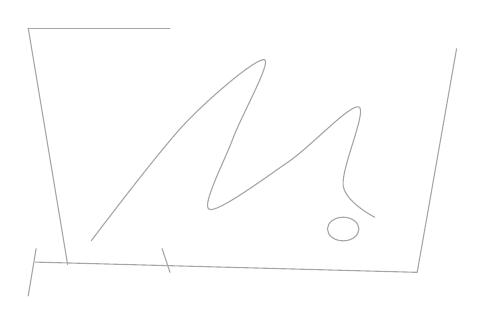
\begin{tikzpicture}[x=1mm,y=1mm,line cap=round,line join=round,font=\scriptsize]
\draw[struck] (12,-16) -- (30,-16);
\draw[struck] (12,-16) -- (17,-46);
\draw[struck] (12.9,-45.7) -- (61.4,-47) -- (66.4,-18.6);
\draw[struck] plot[smooth, tension=0.55] coordinates {(20,-43) (32,-28) (42,-20) (38,-30) (35,-39) (45,-33) (54,-26) (52,-36) (56,-40)};
\draw[struck] (52,-41.5) ellipse[x radius=2, y radius=1.5];
\draw[struck] (13,-44) -- (12,-50);
\draw[struck] (29,-44) -- (30,-47);
\end{tikzpicture}
\end{document}
